%\documentclass[spanish]{beamer}

\documentclass{beamer}
\usepackage{pgf,pgfpages}
%\pgfpagesuselayout{4 on 1}[letterpaper,landscape,border shrink=0.5in]
\usepackage{algorithm,algorithmic}
%\usepackage{algorithm,algorithmicx}
%\usepackage[noend]{algpseudocode}
\usepackage{listings}
\lstset{basicstyle=\ttfamily,
	showstringspaces=false,
	commentstyle=\color{red},
	literate={á}{{\'a}}1
	{ã}{{\~a}}1
	{é}{{\'e}}1
	{É}{{\'E}}1
	{ó}{{\'o}}1
	{í}{{\'i}}1
	{ñ}{{\~n}}1
	{¡}{{!`}}1
	{¿}{{?`}}1
	{ú}{{\'u}}1
	{Í}{{\'I}}1
	{Ó}{{\'O}}1
}

\usepackage{beamerthemesplit}
\usepackage{color}
\usepackage[utf8]{inputenc}
\usepackage[spanish]{babel}
%\usepackage[latin1]{inputenc}
%\usepackage[pdftex]{graphicx}
%\usepackage{algorithm}
%\usepackage{algorithmic-C}
%\usepackage{algorithmic}
\usepackage{amsthm}
\usepackage{multicol}
\usepackage{multirow}
\usepackage{fancyvrb,relsize}
\usepackage{hhline}
\usepackage{tikz}
\usetikzlibrary{trees, shapes, calc}
\newcommand{\inputTikZ}[2]{%
	\scalebox{#1}{\input{#2}}
}

\usetheme{Warsaw} %Gueno
%\usetheme{Darmstadt} %OK!
% \usetheme{Frankfurt} %OK!
%\usetheme{Goettingen}
%\usetheme{Dresden}
%\usetheme{JuanLesPins} %OK!!
%\usetheme{Marburg}
%\usetheme{Montpellier}
%\usetheme{Rochester} %sobrio
%\usetheme{Singapore}
%\usetheme{Szeged}

%\usecolortheme{albatross}
%\usecolortheme{seahorse}
%\usecolortheme{beetle}
%\usecolortheme{crane}
%\usecolortheme{dolphin}
%\usecolortheme{dove}
%\usecolortheme{fly}
%\usecolortheme{lily} %Gueno
\usecolortheme{orchid}%Gueno
%\usecolortheme{rose}
%\usecolortheme{seagull}
%\usecolortheme{whale}


\DefineVerbatimEnvironment%
      {VerbatimNN}%
      {Verbatim}%
      {fontsize=\relsize{-1}}
\DefineVerbatimEnvironment%
      {VerbatimNNN}%
      {Verbatim}%
      {fontsize=\relsize{-2}}

\DefineVerbatimEnvironment%
      {VerbatimPseudo}%
      {Verbatim}%
      {numbers=left, fontsize=\relsize{-1}}
\DefineVerbatimEnvironment%
      {VerbatimPseudoReduced}%
      {Verbatim}%
      {numbers=left, fontsize=\relsize{-2}}
\DefineVerbatimEnvironment%
      {VerbatimPseudoReduced2}%
      {Verbatim}%
      {numbers=left, fontsize=\relsize{-3}}
\DefineVerbatimEnvironment%
      {VerbatimC}%
      {Verbatim}%
      {commandchars=@ªº, numbers=left, fontsize=\relsize{-1}}
\DefineVerbatimEnvironment%
      {VerbatimReducedC}%
      {Verbatim}%
      {commandchars=@ªº, numbers=left, fontsize=\relsize{-2}}
\DefineVerbatimEnvironment%
      {VerbatimReduced2C}%
      {Verbatim}%
      {commandchars=@ªº, numbers=left, fontsize=\relsize{-3}}



%\AtBeginSubsection[]
%{
% \begin{frame}
% \frametitle{Sinopsis}
% Aqui decides: cada seccion y subseccion:
% \tableofcontents[currentsection,currentsubsection]
 %O solamente la seccion (Solo uno de ellos)
%\tableofcontents[currentsection]
% \end{frame}
%}

% Si quieres que todo por default aparezca de poco en poco
% descomenta esta linea
%\beamerdefaultoverlayspecification{<+->}

\setbeamertemplate{footline}{\hfill\insertframenumber/\inserttotalframenumber}
\setbeamertemplate{navigation symbols}{}
\setbeamercovered{transparent}


\title{ELO320 - Estructuras de Datos y Algoritmos\\TDA y Listas Enlazadas}
%\subtitle{Ingeniería Civil Telemática UTFSM}
\author{Dr. Nicolás Gálvez R.\\{\small nicolas.galvez@usm.cl}}
\institute{Ing. Civil Telemática - Departamento de Electrónica}
\titlegraphic{
\includegraphics[scale=.14]{images/logoutfsm}}
\date{1er Semestre 2025}

\begin{document}

\frame{\titlepage}

%\section*{Sinopsis}
%\frame{  \frametitle{Sinopsis}\tableofcontents[pausesections]}
%
%
\section{Tipos de Datos Abstracto (TDA)}

\begin{frame}[fragile]
 \frametitle{TDA: Tipos de Datos Abstracto}
\begin{itemize}
\item \textbf{Tipo de Datos}: Colección de valores y las operaciones que se pueden realizar con éstos. Por ejemplo, enteros (int) con operadores aritméticos. 
\item \textbf{Tipo de Datos Abstracto}: Es una materialización de un tipo de datos como componente de software. Se caracteriza por:
\begin{itemize}
\item Interfaz: conjunto de operaciones.
\item Entradas y salidas interactuan con la interfaz.
\item Implementación oculta.
\item \textbf{La única manera de acceder y manipular los datos del TDA es mediante las operaciones de la interfaz}.
\end{itemize}
\end{itemize}
\end{frame}

\begin{frame}[fragile]
 \frametitle{TDA: Tipos de Datos Abstracto}
\begin{center}
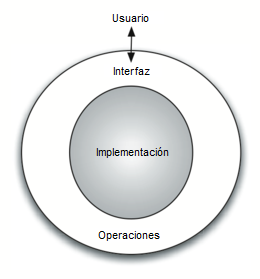
\includegraphics[width=.5\linewidth]{images/tda}\\
\end{center}
\end{frame}

\begin{frame}[fragile]
 \frametitle{TDA: Tipos de Datos Abstracto}
\begin{center}

\includegraphics[width=.6\linewidth]{images/tda_woke}\\
\end{center}

\end{frame}


\section{Lista Enlazada}

\begin{frame}
 \frametitle{Problemas con Arreglos}

\begin{itemize}
\item Los arreglos estáticos ofrecen acceso eficiente a la información.
\item Los arreglos son muy útiles en casos de memoria limitada.
\item Pero, ¿qué pasa con arreglos de forma dinámica?
\begin{itemize}
\item ¿Qué pasa si elimino un elemento del arreglo? {\color{blue}{Debo correr los elementos separados}}.
\item ¿Qué pasa si ingreso un nuevo elemento? {\color{blue}{Debo correr todos los elementos posteriores}}.
\item En el peor de los casos, se deben mover todos los elementos una vez. Por lo tanto serán N instrucciones.
\item Poco eficiente. {\color{red}{$O(n)$}}
\end{itemize}
\item Las listas enlazadas ayudan a manejar esto eficientemente: Simple, Doble y Circular.
\end{itemize}

\end{frame}

\begin{frame}[fragile]
 \frametitle{Lista Simple Enlazada}

Una lista simple enlazada es un TDA que genera un enlace entre nodos a través de punteros. Ventajas:
\begin{itemize}
\item No tienen que estar ordenadas correlativamente en memoria.
\item No es necesario desplazar los elementos en inserciones o eliminaciones. Se modifican los punteros.
\end{itemize}
\begin{center}
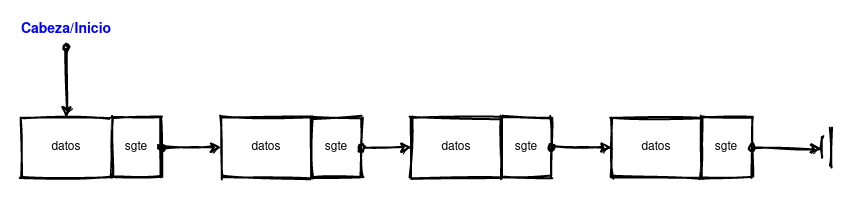
\includegraphics[width=.9\linewidth]{images/linkedlist1}
\end{center}
Está compuesta por:
\begin{itemize}
\item Nodos: Contienen la información en lugares de memoria no ordenados.
\item Punteros: Enlazan los distintos nodos para conformar la lista.
\end{itemize}
\end{frame}

\begin{frame}[fragile]
 \frametitle{Lista Simple Enlazada}

Los punteros permiten al menos:
\begin{itemize}
\item Controlar el inicio de la lista.
\item Apuntar al siguiente elemento en la lista.
\item Acceder a cada nodo.  
\end{itemize}
\begin{center}
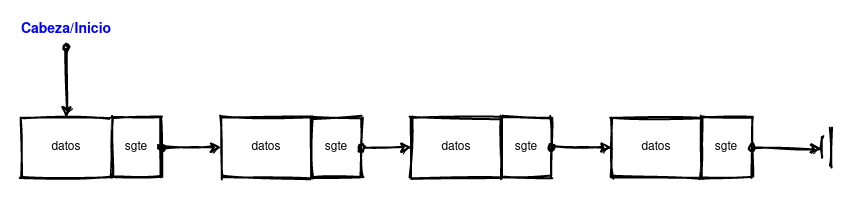
\includegraphics[width=.9\linewidth]{images/linkedlist1}
\end{center}
\end{frame}

\begin{frame}[fragile]
 \frametitle{Lista Simple Enlazada: Nodos}

Los nodos son definidos con un struct, que al menos contiene un tipo de dato y un puntero. 

\begin{exampleblock}{C}
\begin{lstlisting}[language=C, basicstyle=\tiny, escapeinside={|}{|}]
struct nodo{
	int dato; //dato, puede ser lo que uds. necesiten
	struct nodo *sgte; // puntero a un nodo, enlace
};

typedef struct le_nodo{
	float datos[20]; //dato, puede ser lo que uds. necesiten
	struct le_nodo *sgte; // puntero a un nodo, enalce.
} nodo_t;
\end{lstlisting}
\end{exampleblock}
\begin{center}
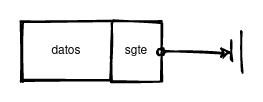
\includegraphics[width=.45\linewidth]{images/node}
\end{center}
\end{frame}


\begin{frame}[fragile]
 \frametitle{Lista Simple Enlazada: Interfaz}

Al igual que Python (\texttt{list()} o \texttt{[]}), las listas tienen un conjunto de funciones que interactúan como interfaz:
\begin{itemize}
\item <1> Inicializar Lista. 
\item <1> Agregar un elemento a una lista. 
\item <1> Determinar el largo de una lista.
\item <1> Eliminar un elemento de una lista.
\item <1> Imprimir una lista. 
\item <1> Limpiar una lista. 
\end{itemize}
\begin{center}
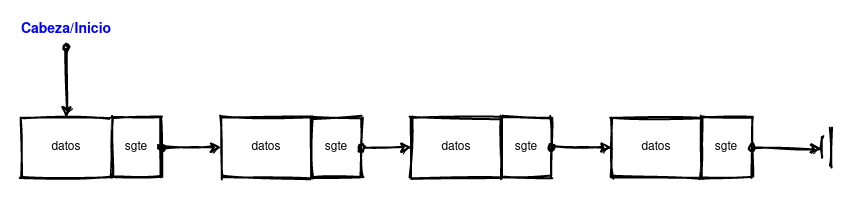
\includegraphics[width=.9\linewidth]{images/linkedlist1}
\end{center}
\end{frame}

\begin{frame}[fragile]
 \frametitle{Lista Simple Enlazada: Interfaz}

Al igual que Python (\texttt{list()} o \texttt{[]}), las listas tienen un conjunto de funciones que interactúan como interfaz:
\begin{itemize}
\item <1> Inicializar Lista. 
\item <1> Agregar un elemento a una lista. 
\item <0> Determinar el largo de una lista.
\item <0> Eliminar un elemento de una lista.
\item <0> Imprimir una lista. 
\item <0> Limpiar una lista. 
\end{itemize}
\begin{center}
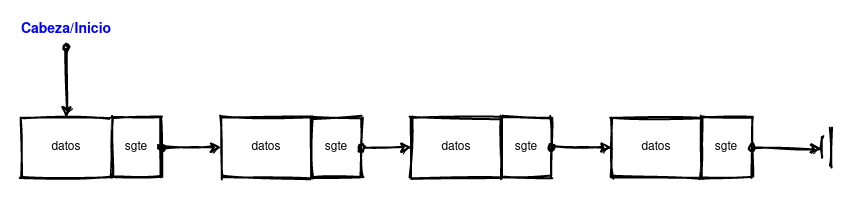
\includegraphics[width=.9\linewidth]{images/linkedlist1}
\end{center}
\end{frame}


\begin{frame}[fragile]
 \frametitle{Lista Simple Enlazada: Inicializar}

Las listas, en su versión más básica, dependen de un puntero al inicio de la lista. Éste suele llamarse \textit{header}, \textit{cabecera} o  \textit{inicio}.
\begin{exampleblock}{C}
\begin{lstlisting}[language=C, basicstyle=\tiny, escapeinside={|}{|}]
#include<stdio.h>

typedef struct nodo{
	int dato; //dato, puede ser lo que uds. necesiten
	struct nodo *sgte; // puntero a un nodo enalce.
} nodo_t;

int main(int argc, char **argv){

	nodo_t * inicio = NULL; 
	// Inicializamos la lista, con su puntero de inicio apuntando a NULL
	// Equivalente a lista vacía []

	return 0;
}
\end{lstlisting}
\end{exampleblock}

\begin{center}

\includegraphics[width=0.3\linewidth]{images/init1}
\end{center}
\end{frame}

\begin{frame}[fragile]
 \frametitle{Lista Simple Enlazada: Añadir nodos}

Tendremos 4 casos a tener en consideración.

\begin{itemize}
\item Añadir primer nodo $\rightarrow$ lista vacía.
\item Añadir al inicio.
\item Añadir entre nodos.
\item Añadir al final.
\end{itemize}

\end{frame}

\begin{frame}[fragile]
 \frametitle{Lista Simple Enlazada: Primer nodo}

Esquema:
\begin{center}
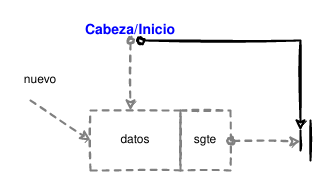
\includegraphics[width=0.45\linewidth]{images/firstadd1}
\end{center}

Debemos: 
\begin{enumerate}
\item<1-> Crear el nodo \texttt{nuevo}.
\item<0> Asignar el dato. 
\item<0> Puntero siguiente de nuevo (\texttt{nuevo->sgte}) apunta a \texttt{NULL}.
\item<0> Puntero \texttt{inicio} apunta a nuevo.
\end{enumerate}
\end{frame}

\begin{frame}[fragile]
 \frametitle{Lista Simple Enlazada: Primer nodo}

Esquema:
\begin{center}
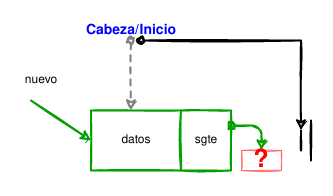
\includegraphics[width=0.45\linewidth]{images/firstadd2}
\end{center}

Debemos: 
\begin{enumerate}
\item<1> Crear el nodo \texttt{nuevo}.
\item<1> Asignar el dato. 
\item<0> Puntero siguiente de nuevo (\texttt{nuevo->sgte}) apunta a \texttt{NULL}.
\item<0> Puntero \texttt{inicio} apunta a nuevo.
\end{enumerate}

\end{frame}

\begin{frame}[fragile]
 \frametitle{Lista Simple Enlazada: Primer nodo}

Esquema:
\begin{center}
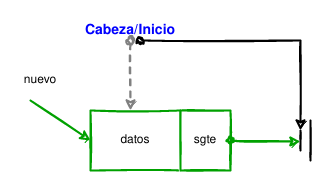
\includegraphics[width=0.45\linewidth]{images/firstadd3}
\end{center}

Debemos: 
\begin{enumerate}
\item<1> Crear el nodo \texttt{nuevo}.
\item<1> Asignar el dato. 
\item<1> Puntero siguiente de nuevo (\texttt{nuevo->sgte}) apunta a \texttt{NULL}.
\item<0> Puntero \texttt{inicio} apunta a nuevo.
\end{enumerate}

\end{frame}


\begin{frame}[fragile]
 \frametitle{Lista Simple Enlazada: Primer nodo}

Esquema:
\begin{center}
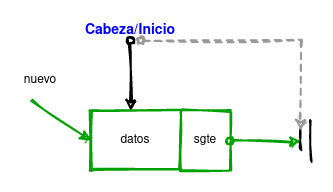
\includegraphics[width=0.45\linewidth]{images/firstadd4}
\end{center}

Debemos: 
\begin{enumerate}
\item<1> Crear el nodo \texttt{nuevo}.
\item<1> Asignar el dato. 
\item<1> Puntero siguiente de nuevo (\texttt{nuevo->sgte}) apunta a \texttt{NULL}.
\item<1> Puntero \texttt{inicio} apunta a nuevo.
\end{enumerate}

\end{frame}



\begin{frame}[fragile]
 \frametitle{Lista Simple Enlazada: Primer nodo}
\begin{center}
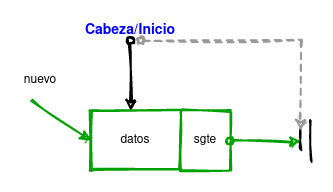
\includegraphics[width=0.45\linewidth]{images/firstadd4}
\end{center}

\begin{exampleblock}{C}
\begin{lstlisting}[language=C, basicstyle=\tiny, escapeinside={|}{|}]
/* No complicarse: ** = puntero pasado por referencia
para que dirección de memoria cambie afuera de la función */
void first_node(nodo_t **cabeza, int dato){ 

        nodo_t *nuevo = malloc(sizeof(nodo_t)); // 1) crea nodo
	nuevo->dato = dato; // 2) asigna dato
	nuevo->sgte = NULL; // 3) siguiente apunta a NULL
	*cabeza = nuevo; // 4) inicio apunta a nuevo 
}
\end{lstlisting}
\end{exampleblock}
\end{frame}

\begin{frame}[fragile]
 \frametitle{Lista Simple Enlazada: Añadir al inicio}
Esquema:
\begin{center}
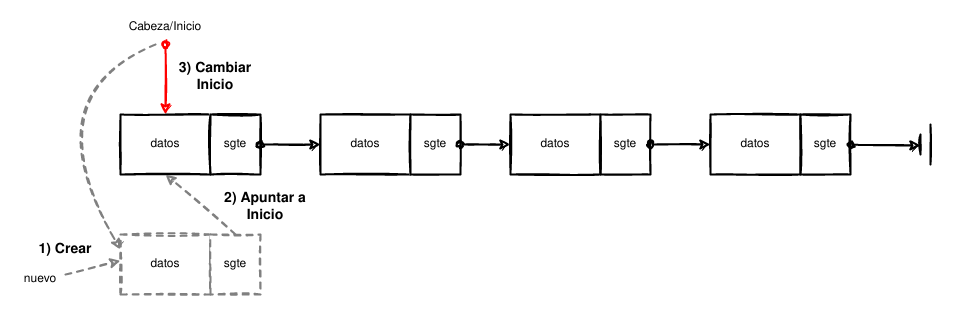
\includegraphics[width=0.9\linewidth]{images/addheader1}
\end{center}

Debemos: 
\begin{enumerate}
\item<1> Crear el nodo \texttt{nuevo}.
\item<0> Asignar el dato. 
\item<0> Puntero siguiente de nuevo (\texttt{nuevo->sgte}) apunta a \texttt{inicio}.
\item<0> Puntero \texttt{inicio} apunta a nuevo.
\end{enumerate}

\end{frame}

\begin{frame}[fragile]
 \frametitle{Lista Simple Enlazada: Añadir al inicio}
Esquema:
\begin{center}
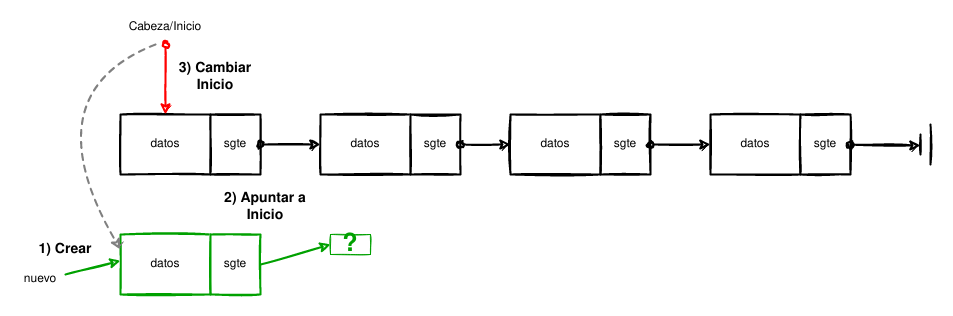
\includegraphics[width=0.9\linewidth]{images/addheader2}
\end{center}

Debemos: 
\begin{enumerate}
\item<1> Crear el nodo \texttt{nuevo}.
\item<1> Asignar el dato. 
\item<0> Puntero siguiente de nuevo (\texttt{nuevo->sgte}) apunta a \texttt{inicio}.
\item<0> Puntero \texttt{inicio} apunta a nuevo.
\end{enumerate}

\end{frame}

\begin{frame}[fragile]
 \frametitle{Lista Simple Enlazada: Añadir al inicio}
Esquema:
\begin{center}
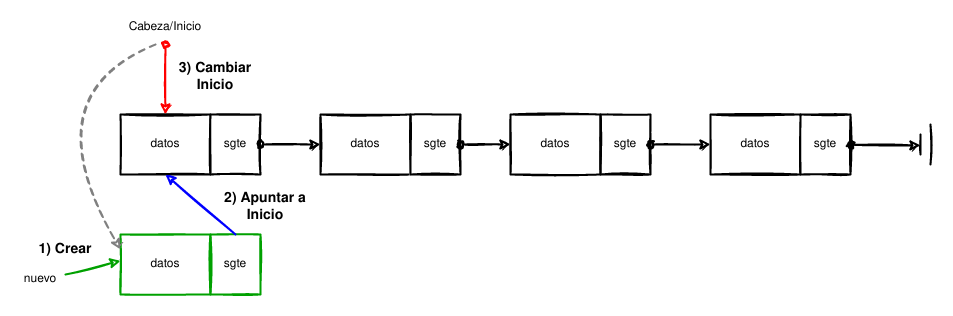
\includegraphics[width=0.9\linewidth]{images/addheader3}
\end{center}

Debemos: 
\begin{enumerate}
\item<1> Crear el nodo \texttt{nuevo}.
\item<1> Asignar el dato. 
\item<1> Puntero siguiente de nuevo (\texttt{nuevo->sgte}) apunta a \texttt{inicio}.
\item<0> Puntero \texttt{inicio} apunta a nuevo.
\end{enumerate}

\end{frame}

\begin{frame}[fragile]
 \frametitle{Lista Simple Enlazada: Añadir al inicio}
Esquema:
\begin{center}
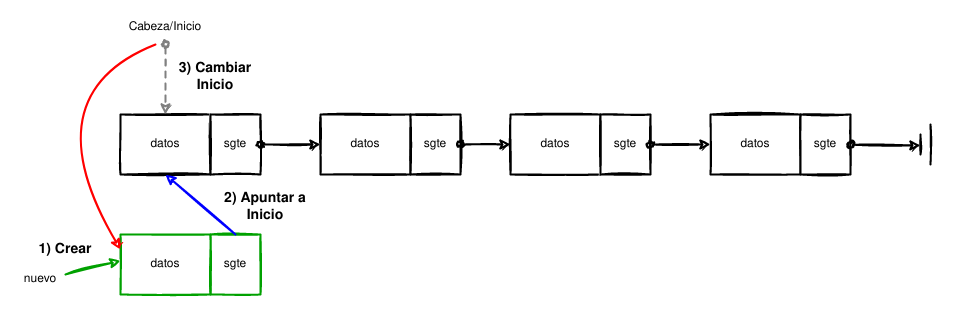
\includegraphics[width=0.9\linewidth]{images/addheader4}
\end{center}

Debemos: 
\begin{enumerate}
\item<1> Crear el nodo \texttt{nuevo}.
\item<1> Asignar el dato. 
\item<1> Puntero siguiente de nuevo (\texttt{nuevo->sgte}) apunta a \texttt{inicio}.
\item<1> Puntero \texttt{inicio} apunta a nuevo.
\end{enumerate}

\end{frame}

\begin{frame}[fragile]
 \frametitle{Lista Simple Enlazada: Añadir al inicio}
\begin{center}
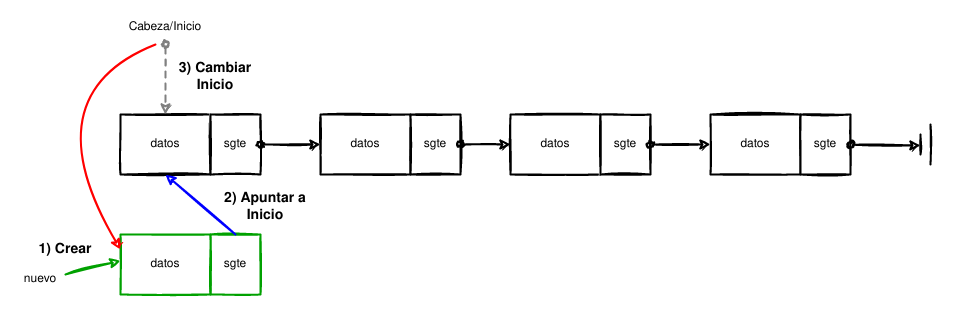
\includegraphics[width=0.9\linewidth]{images/addheader4}
\end{center}

\begin{exampleblock}{C}
\begin{lstlisting}[language=C, basicstyle=\tiny, escapeinside={|}{|}]
void add_first(nodo_t **cabeza, int dato){ 	          

	nodo_t *nuevo = malloc(sizeof(nodo_t)); // 1) crea nodo
	nuevo->dato = dato; // 2) asigna dato
	nuevo->sgte = *cabeza; // 3) siguiente apunta a inicio
	*cabeza = nuevo; // 4) inicio apunta a nuevo 
}
\end{lstlisting}
\end{exampleblock}

\end{frame}

\begin{frame}[fragile]
 \frametitle{Lista Simple Enlazada: Añadir entre nodos}
Esquema:
\begin{center}
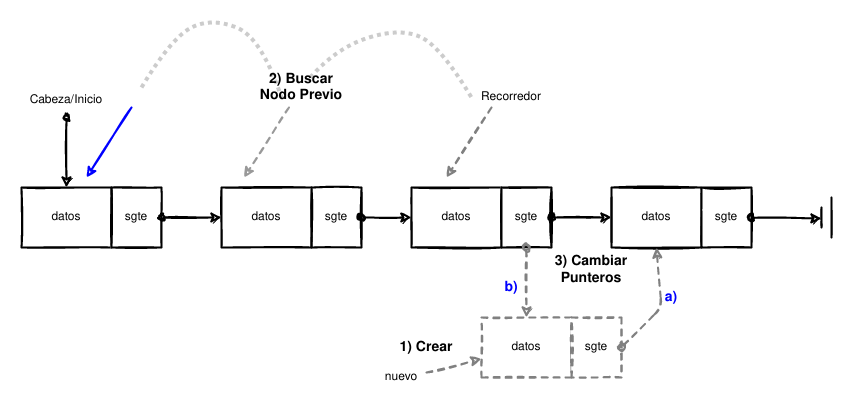
\includegraphics[width=0.8\linewidth]{images/addmiddle1}
\end{center}

Debemos: 
\begin{enumerate}
\item<1> Crear el nodo \texttt{nuevo}.
\item<0> Asignar el dato. 
\item<0> Buscar nodo previo al objetivo: por valor o posición. 
\item<0> Cambiar punteros.
\end{enumerate}

\end{frame}

\begin{frame}[fragile]
 \frametitle{Lista Simple Enlazada: Añadir entre nodos}
Esquema:
\begin{center}
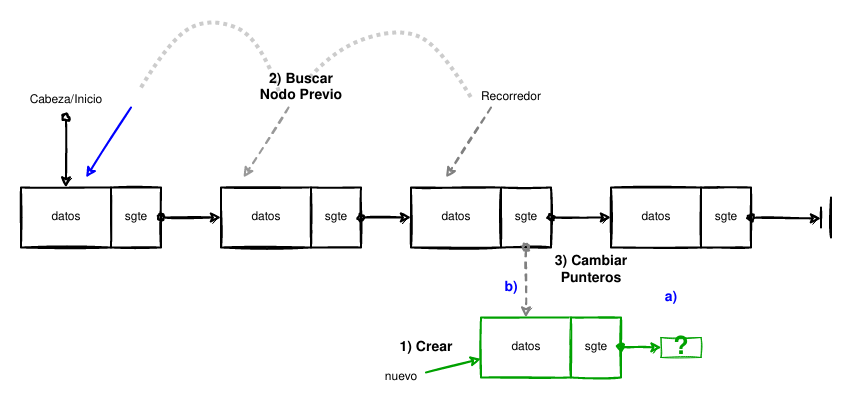
\includegraphics[width=0.8\linewidth]{images/addmiddle2}
\end{center}

Debemos: 
\begin{enumerate}
\item<1> Crear el nodo \texttt{nuevo}.
\item<1> Asignar el dato. 
\item<0> Buscar nodo previo al objetivo: por valor o posición. 
\item<0> Cambiar punteros.
\end{enumerate}

\end{frame}

\begin{frame}[fragile]
 \frametitle{Lista Simple Enlazada: Añadir entre nodos}
Esquema:
\begin{center}
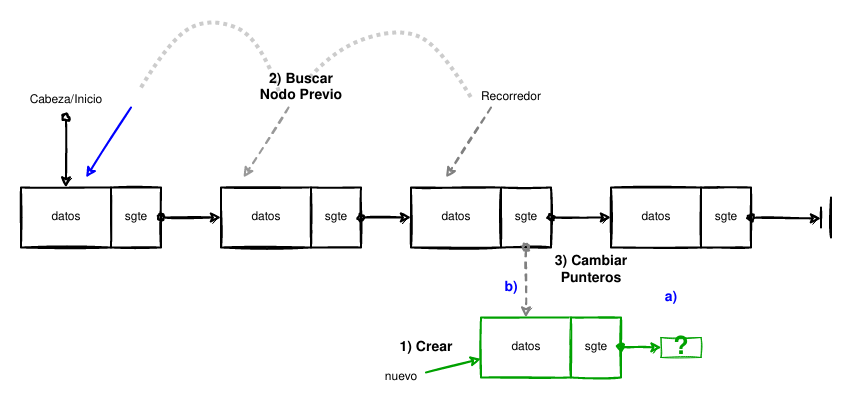
\includegraphics[width=0.8\linewidth]{images/addmiddle2}
\end{center}

Debemos: 
\begin{enumerate}
\item<1> Crear el nodo \texttt{nuevo}.
\item<1> Asignar el dato. 
\item<1> Buscar nodo previo al objetivo: por valor o posición. 
\item<0> Cambiar punteros.
\end{enumerate}

\end{frame}

\begin{frame}[fragile]
 \frametitle{Lista Simple Enlazada: Añadir entre nodos}
Esquema:
\begin{center}
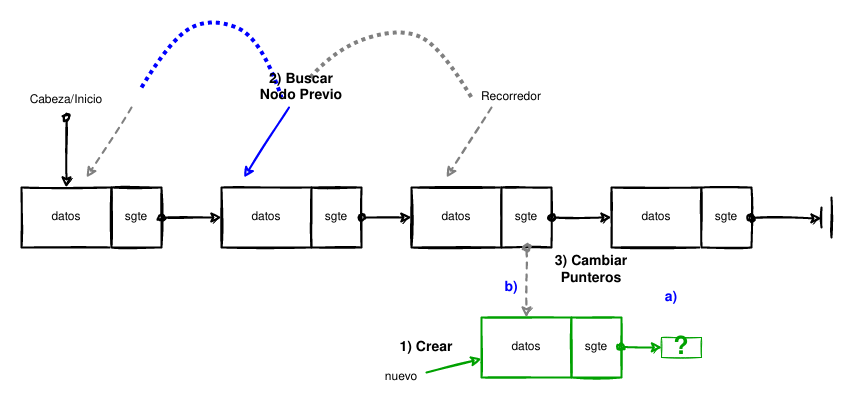
\includegraphics[width=0.8\linewidth]{images/addmiddle3}
\end{center}

Debemos: 
\begin{enumerate}
\item<1> Crear el nodo \texttt{nuevo}.
\item<1> Asignar el dato. 
\item<1> Buscar nodo previo al objetivo: por valor o posición. 
\item<0> Cambiar punteros.
\end{enumerate}

\end{frame}

\begin{frame}[fragile]
 \frametitle{Lista Simple Enlazada: Añadir entre nodos}
Esquema:
\begin{center}
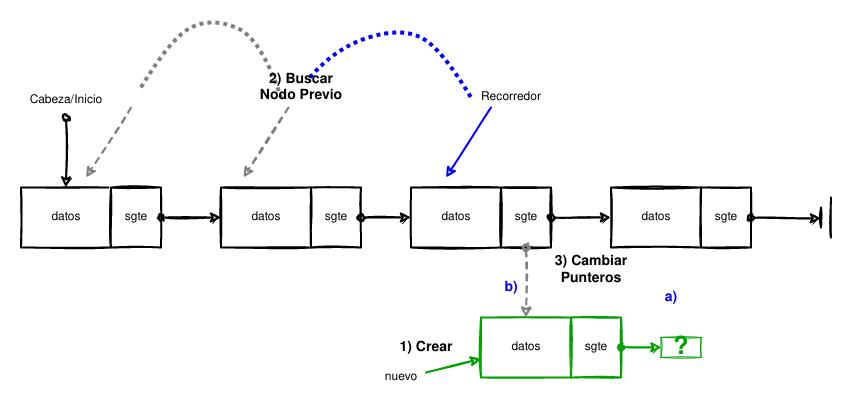
\includegraphics[width=0.8\linewidth]{images/addmiddle4}
\end{center}

Debemos: 
\begin{enumerate}
\item<1> Crear el nodo \texttt{nuevo}.
\item<1> Asignar el dato. 
\item<1> Buscar nodo previo al objetivo: por valor o posición. 
\item<0> Cambiar punteros.
\end{enumerate}

\end{frame}

\begin{frame}[fragile]
 \frametitle{Lista Simple Enlazada: Añadir entre nodos}
Esquema:
\begin{center}
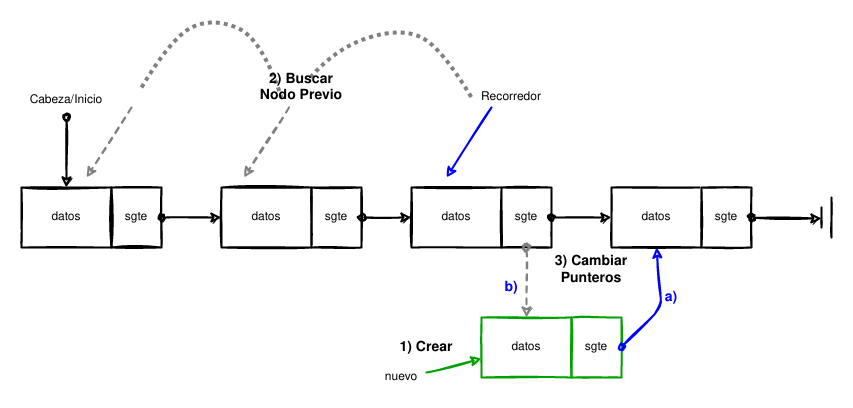
\includegraphics[width=0.8\linewidth]{images/addmiddle5}
\end{center}

Debemos: 
\begin{enumerate}
\item<1> Crear el nodo \texttt{nuevo}.
\item<1> Asignar el dato. 
\item<1> Buscar nodo previo al objetivo: por valor o posición. 
\item<1> Cambiar punteros.
\end{enumerate}

\end{frame}

\begin{frame}[fragile]
 \frametitle{Lista Simple Enlazada: Añadir entre nodos}
Esquema:
\begin{center}
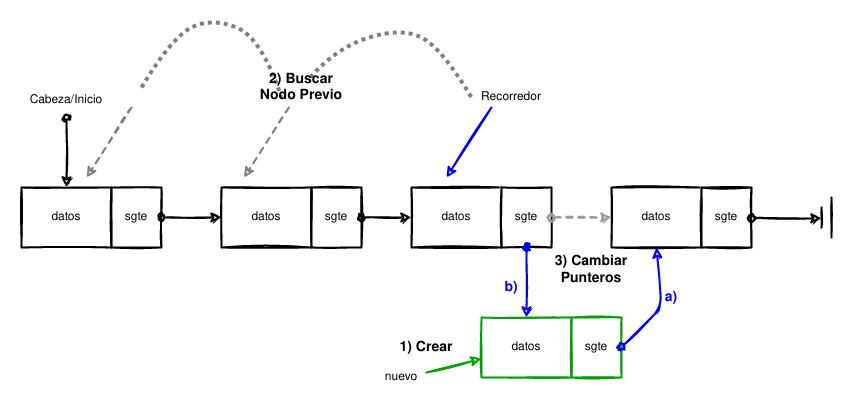
\includegraphics[width=0.8\linewidth]{images/addmiddle6}
\end{center}

Debemos: 
\begin{enumerate}
\item<1> Crear el nodo \texttt{nuevo}.
\item<1> Asignar el dato. 
\item<1> Buscar nodo previo al objetivo: por valor o posición. 
\item<1> Cambiar punteros.
\end{enumerate}

\end{frame}



\begin{frame}[fragile]
 \frametitle{Lista Simple Enlazada: Añadir entre nodos}
\begin{center}
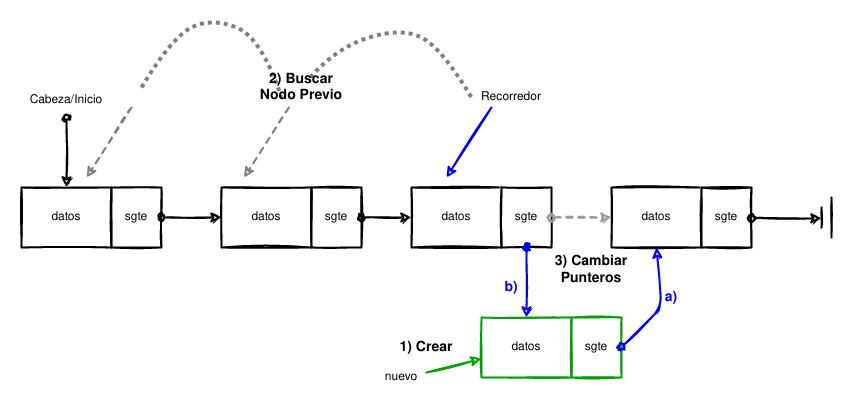
\includegraphics[width=0.5\linewidth]{images/addmiddle6}
\end{center}

\begin{exampleblock}{C}
\begin{lstlisting}[language=C, basicstyle=\tiny, escapeinside={|}{|}]
// no se modifica el puntero inicio, no es necesario el **
void add_middle(nodo_t *cabeza, int dato, int pos){ 	          

	nodo_t *nuevo = malloc(sizeof(nodo_t)); // 1) crea nodo
	nuevo->dato = dato; // 2) asigna dato

	int cont; // nos ayudará a ver la posición en que estamos
	nodo_t *recorredor = cabeza; // ptr que recorre la lista.
	
	for(cont=0; cont<pos-1; cont ++){ //pos-1, para encontrar el previo
		recorredor = recorredor->sgte; //avanza al siguiente nodo
	} // 3) al finalizar el for, tenemos el nodo previo identificado

	nuevo->sgte = recorredor->sgte; // 4) cambio de punteros
	recorredor->sgte = nuevo; // El orden importa. Memory Leak!
}
\end{lstlisting}
\end{exampleblock}

\end{frame}

\begin{frame}[fragile]
 \frametitle{Lista Simple Enlazada: Añadir al final.}
Esquema:
\begin{center}
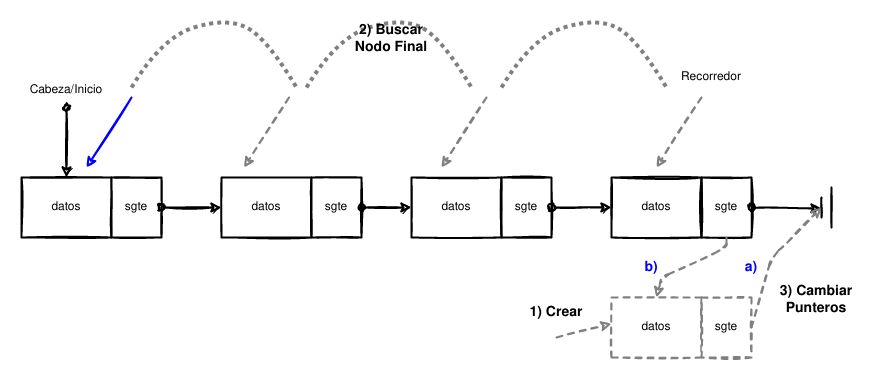
\includegraphics[width=0.8\linewidth]{images/append1}
\end{center}

Debemos: 
\begin{enumerate}
\item<1> Crear el nodo \texttt{nuevo}.
\item<0> Asignar el dato. 
\item<0> Buscar nodo final. 
\item<0> Cambiar punteros.
\end{enumerate}

\end{frame}

\begin{frame}[fragile]
 \frametitle{Lista Simple Enlazada: Añadir al final.}
Esquema:
\begin{center}
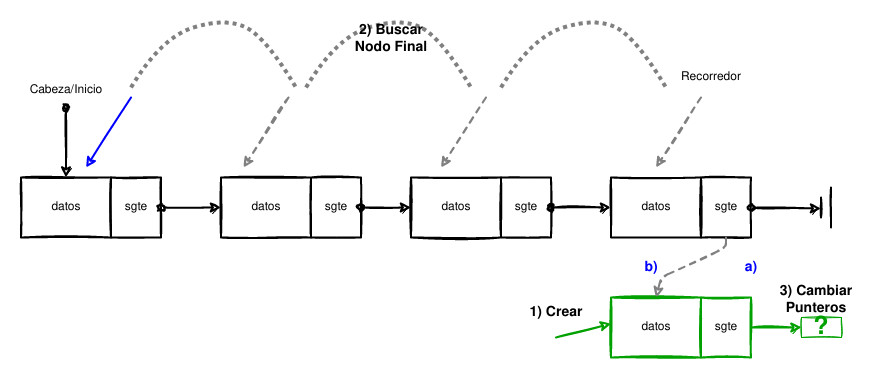
\includegraphics[width=0.8\linewidth]{images/append2}
\end{center}

Debemos: 
\begin{enumerate}
\item<1> Crear el nodo \texttt{nuevo}.
\item<1> Asignar el dato. 
\item<0> Buscar nodo final. 
\item<0> Cambiar punteros.
\end{enumerate}

\end{frame}

\begin{frame}[fragile]
 \frametitle{Lista Simple Enlazada: Añadir al final.}
Esquema:
\begin{center}
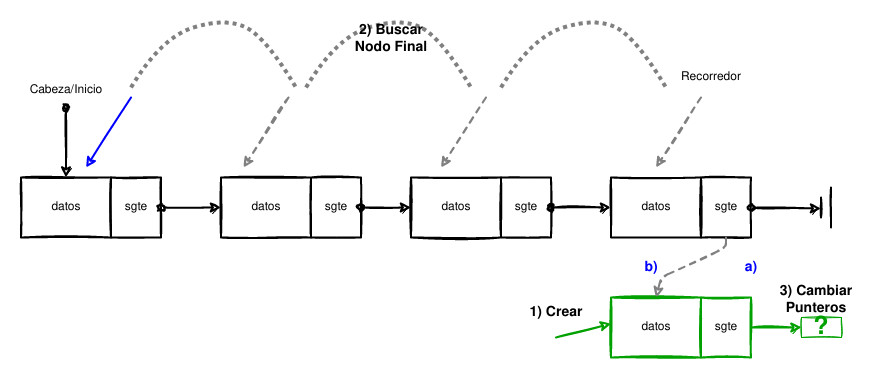
\includegraphics[width=0.8\linewidth]{images/append2}
\end{center}

Debemos: 
\begin{enumerate}
\item<1> Crear el nodo \texttt{nuevo}.
\item<1> Asignar el dato. 
\item<1> Buscar nodo final. 
\item<0> Cambiar punteros.
\end{enumerate}

\end{frame}

\begin{frame}[fragile]
 \frametitle{Lista Simple Enlazada: Añadir al final.}
Esquema:
\begin{center}
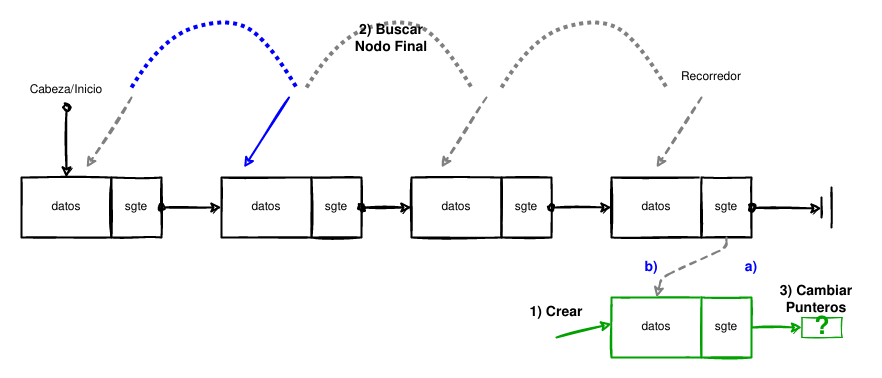
\includegraphics[width=0.8\linewidth]{images/append3}
\end{center}

Debemos: 
\begin{enumerate}
\item<1> Crear el nodo \texttt{nuevo}.
\item<1> Asignar el dato. 
\item<1> Buscar nodo final. 
\item<0> Cambiar punteros.
\end{enumerate}

\end{frame}

\begin{frame}[fragile]
 \frametitle{Lista Simple Enlazada: Añadir al final.}
Esquema:
\begin{center}
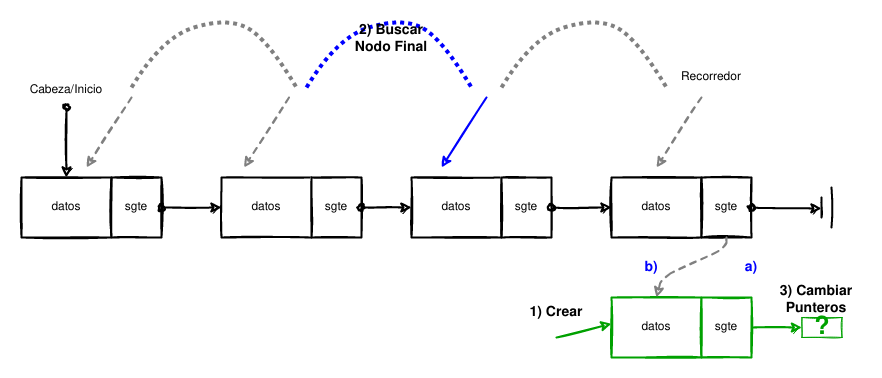
\includegraphics[width=0.8\linewidth]{images/append4}
\end{center}

Debemos: 
\begin{enumerate}
\item<1> Crear el nodo \texttt{nuevo}.
\item<1> Asignar el dato. 
\item<1> Buscar nodo final. 
\item<0> Cambiar punteros.
\end{enumerate}

\end{frame}

\begin{frame}[fragile]
 \frametitle{Lista Simple Enlazada: Añadir al final.}
Esquema:
\begin{center}
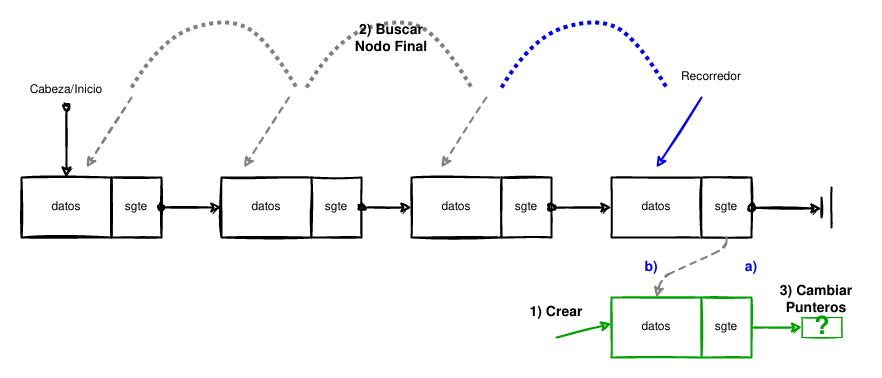
\includegraphics[width=0.8\linewidth]{images/append5}
\end{center}

Debemos: 
\begin{enumerate}
\item<1> Crear el nodo \texttt{nuevo}.
\item<1> Asignar el dato. 
\item<1> Buscar nodo final. 
\item<0> Cambiar punteros.
\end{enumerate}

\end{frame}

\begin{frame}[fragile]
 \frametitle{Lista Simple Enlazada: Añadir al final.}
Esquema:
\begin{center}
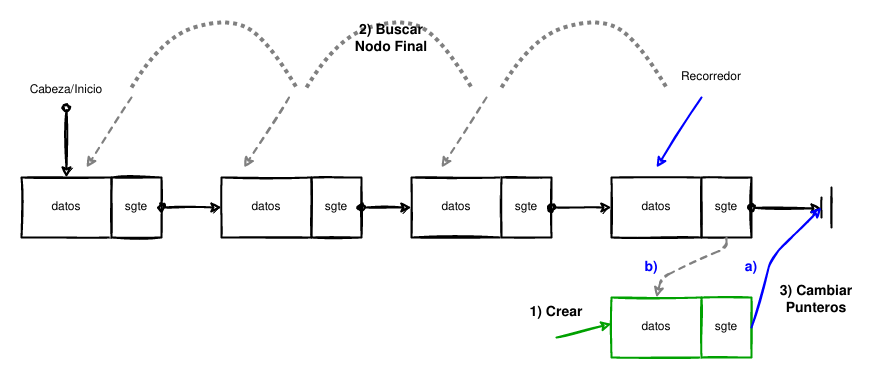
\includegraphics[width=0.8\linewidth]{images/append6}
\end{center}

Debemos: 
\begin{enumerate}
\item<1> Crear el nodo \texttt{nuevo}.
\item<1> Asignar el dato. 
\item<1> Buscar nodo final. 
\item<1> Cambiar punteros.
\end{enumerate}

\end{frame}

\begin{frame}[fragile]
 \frametitle{Lista Simple Enlazada: Añadir al final.}
Esquema:
\begin{center}
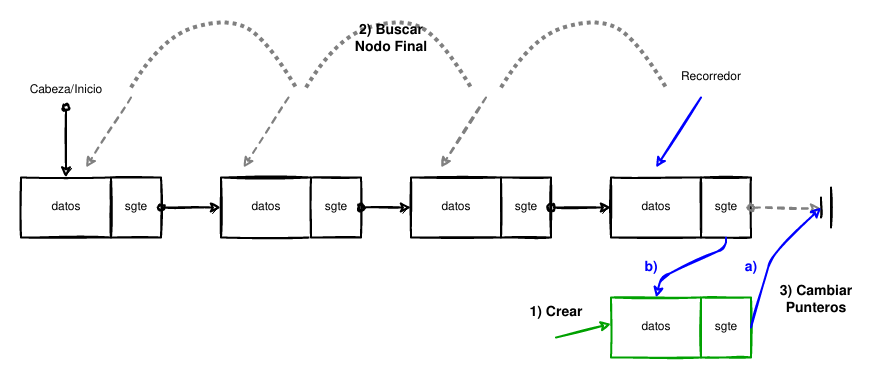
\includegraphics[width=0.8\linewidth]{images/append7}
\end{center}

Debemos: 
\begin{enumerate}
\item<1> Crear el nodo \texttt{nuevo}.
\item<1> Asignar el dato. 
\item<1> Buscar nodo final. 
\item<1> Cambiar punteros.
\end{enumerate}

\end{frame}


\begin{frame}[fragile]
 \frametitle{Lista Simple Enlazada: Añadir al final}
\begin{center}
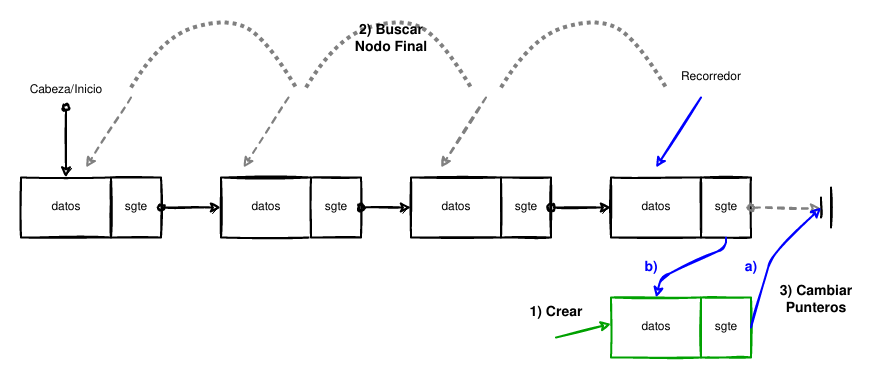
\includegraphics[width=0.5\linewidth]{images/append7}
\end{center}

\begin{exampleblock}{C}
\begin{lstlisting}[language=C, basicstyle=\tiny, escapeinside={|}{|}]
void append(nodo_t *cabeza, int dato){ 	          

	nodo_t *nuevo = malloc(sizeof(nodo_t)); // 1) crea nodo
	nuevo->dato = dato; // 2) asigna dato

	nodo_t *recorredor = cabeza; // ptr que recorre la lista.
	while(recorredor->sgte!=NULL){
		recorredor=recorredor->sgte; // 3) avanzamos hasta llegar al final
	}

	nuevo->sgte = recorredor->sgte; // 4) cambio de punteros
	recorredor->sgte = nuevo; // El orden importa. Memory Leak!
}
\end{lstlisting}
\end{exampleblock}

\end{frame}

\begin{frame}[fragile]
 \frametitle{Lista Simple Enlazada: Añadir general}

\begin{exampleblock}{C}
\begin{lstlisting}[language=C, basicstyle=\tiny]
void add_node(nodo_t **cabeza, int dato, int pos){ 	          
	nodo_t * nuevo = malloc(sizeof(nodo_t));
	nodo_t * recorredor = (*cabeza);
	int cont;

	if (nuevo == NULL){
		printf("Error en creación de nodo\n");
		exit(-1);
	}
	nuevo->dato = dato;

	if(recorredor==NULL || pos==0){ //casos primer nodo
		nuevo->sgte=(*cabeza);
		*cabeza = nuevo;
	}else{ //caso entre nodos y final
		for(cont=0; cont<pos-1; cont++){
			if(recorredor->sgte == NULL) //para nodo final
				break; 
			recorredor = recorredor->sgte;
		}
		nuevo->sgte = recorredor->sgte;
		recorredor->sgte = nuevo;
	}
}
\end{lstlisting}
\end{exampleblock}
\end{frame}

\begin{frame}[fragile]
 \frametitle{Lista Simple Enlazada: Interfaz}

Al igual que Python (\texttt{list()} o \texttt{[]}), las listas tienen un conjunto de funciones que interactúan como interfaz:
\begin{itemize}
\item <0> Inicializar Lista. 
\item <0> Agregar un elemento a una lista. 
\item <1> Determinar el largo de una lista.
\item <1> Eliminar un elemento de una lista.
\item <1> Imprimir una lista. 
\item <1> Limpiar una lista. 
\end{itemize}
\begin{center}
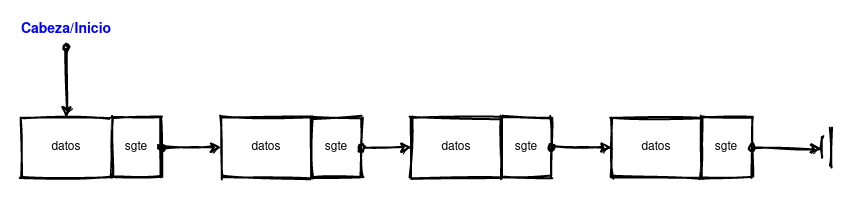
\includegraphics[width=.9\linewidth]{images/linkedlist1}
\end{center}
\end{frame}
%
%\begin{frame}[fragile]
% \frametitle{Lista Simple Enlazada: Largo de lista.}
%
%Seguramente, considerarían más sencillas las funciones anteriores si tuvieremos el largo de la lista. Siguiendo el principio de recorrer:
%
%\begin{center}
%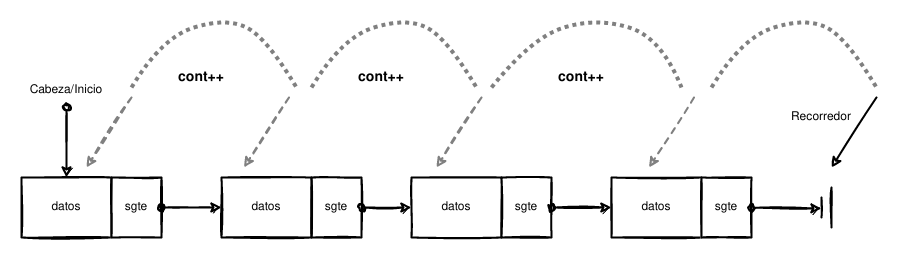
\includegraphics[width=.9\linewidth]{images/length}
%\end{center}
%
%\begin{exampleblock}{C}
%\begin{lstlisting}[language=C, basicstyle=\tiny, escapeinside={|}{|}]
%int list_len(nodo_t *cabeza){ 	          
%
%	nodo_t *recorredor = cabeza;
%	int cont;
%
%	for(cont=0; recorredor!=NULL; cont++){
%		recorredor = recorredor -> sgte;
%	}
%	
%	return cont;
%}
%\end{lstlisting}
%\end{exampleblock}
%
%\end{frame}
%
%\begin{frame}[fragile]
% \frametitle{Lista Simple Enlazada: Eliminar nodos}
%
%Tendremos 2 casos a tener en consideración. Uds, deberán implementarlos a partir de las figuras.
%
%\begin{itemize}
%\item Eliminar primer nodo.
%\item Eliminar nodo intermedio o final.
%\end{itemize}
%
%Ojo, que no siempre se pueden borrar nodos: \textbf{lista vacía}.
%
%\end{frame}
%
%\begin{frame}[fragile]
% \frametitle{Lista Simple Enlazada: Eliminar primero nodo}
%
%Implemente la siguiente figura:
%
%\begin{center}
%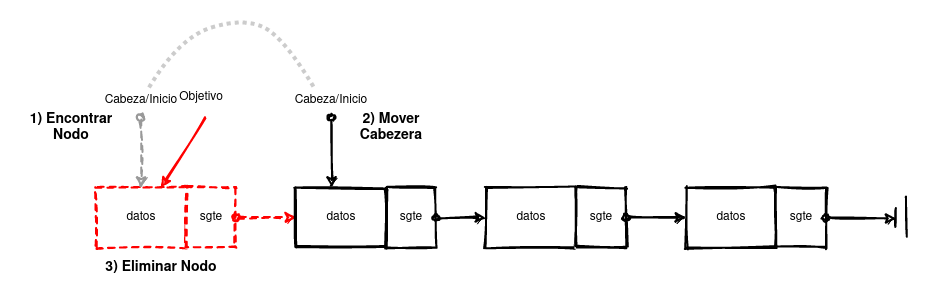
\includegraphics[width=.9\linewidth]{images/deleteheader}
%\end{center}
%
%Ojo, que no siempre se pueden borrar nodos: \textbf{lista vacía}.
%
%\end{frame}
%
%\begin{frame}[fragile]
% \frametitle{Lista Simple Enlazada: Eliminar nodo intermedio o final}
%
%Implemente la siguiente figura:
%
%\begin{center}
%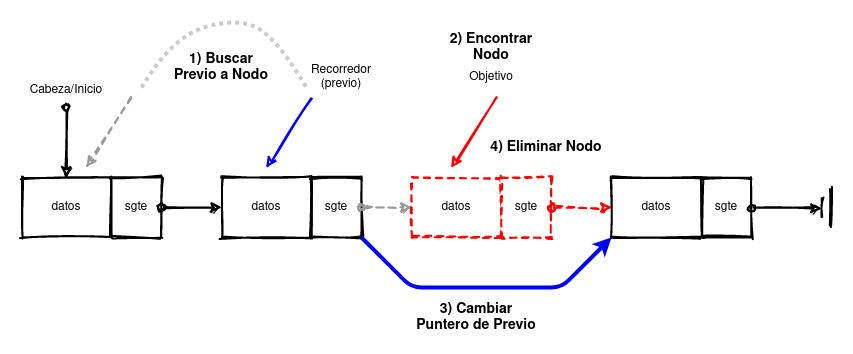
\includegraphics[width=.9\linewidth]{images/delete}
%\end{center}
%
%Ojo, que no siempre se pueden borrar nodos: \textbf{lista vacía}.
%
%\end{frame}
%
%
%\begin{frame}[fragile]
% \frametitle{Lista Simple Enlazada: Imprimir Lista.}
%
%Para verificar que la lista está en cierto estado, pueden crear la función imprimir lista. Explique como funciona con una figura.
%
%\begin{exampleblock}{C}
%\begin{lstlisting}[language=C, basicstyle=\tiny, escapeinside={|}{|}]
%void print_list(nodo_t *cabeza){ 	          
%
%	// rec = recorredor ;)
%	nodo_t *rec = cabeza;
%	int cont;
%
%	printf("--- Print Lista ---\n");
%	for(cont=0; rec!=NULL; cont++){
%		printf("Lista pos |\%|d, valor: |\%|d\n", cont, rec->dato);
%		rec = rec -> sgte;
%	}
%	printf("--- Fin Lista ---\n\n");
%	
%}
%\end{lstlisting}
%\end{exampleblock}
%
%\end{frame}
%
%\begin{frame}[fragile]
% \frametitle{Lista Simple Enlazada: Limpiar Lista.}
%
%Recuerden que al final de cada uso, toda la memoria reservada \textbf{debe ser liberada}. Por lo tanto, esta función es obligatoria. Explique como funciona con una figura.
%
%\begin{exampleblock}{C}
%\begin{lstlisting}[language=C, basicstyle=\tiny, escapeinside={|}{|}]
%void free_list(nodo_t *cabeza){ 	          
%
%	// rec = recorredor ;)
%	nodo_t *rec = cabeza;
%
%	while(rec!=NULL){
%		cabeza = rec->sgte;
%		free(rec);
%		rec=cabeza;
%	}
%	//¿qué le pasa al puntero cabecera?
%	//¿cómo lo arreglan?
%}
%\end{lstlisting}
%\end{exampleblock}
%
%\end{frame}
%
%
%\section{Problemas con punteros.}
%
%\frame[containsverbatim]
%{
%\frametitle{Dangling}
%\begin{itemize}
%\item \textbf{Dejar Colgado (dangling).} 
%\item Puntero hacia localización de memoria del heap que ha sido liberada (e incluso nuevamente asignada). 
%\item Genera errores poco predecibles (e.g. Segmentation fault, corrupción de memoria).
%\end{itemize}
%\begin{exampleblock}{C}
%\begin{lstlisting}[language=C, basicstyle=\tiny, escapeinside={|}{|}]
%int main(int argc, char **argv){
%	int x=2;
%	int *p, *q;
%
%	p= malloc(sizeof(int));
%	q=p;
%
%	free(p);  /* q aun mantiene referencia al heap */
%        	 /* puede que variable de heap sea reasignada */
%
%	*q = x;
%
%	return 0;
%}
%\end{lstlisting}
%\end{exampleblock}
%}
%
%
%\frame[containsverbatim]
%{
%\frametitle{Fuga de memoria - Memory Leak}
%\begin{itemize}
%\item \textbf{Fuga de memoria (memory leak)}. 
%\item Pérdida de acceso a objeto de memoria reservado en el heap, por no existir variables que apunten a él. 
%\item No se puede liberar hasta el término del programa.
%\item Puede saturar la memoria.
%\end{itemize}
%\begin{exampleblock}{C}
%\begin{lstlisting}[language=C, basicstyle=\tiny, escapeinside={|}{|}]
%int main(int argc, char **argv){
%	int *p;
%	
%	p= malloc(sizeof(int));
%	p= malloc(sizeof(int));
%	/* se pierde la direccion asignada anteriormente */
%
%	free(p);
%
%	return 0;
%\end{lstlisting}
%\end{exampleblock}
%}
%
%
%\frame[containsverbatim]
%{
%\frametitle{Ejemplo}
%
%\begin{center}
%{\centering \Large Dangling}
%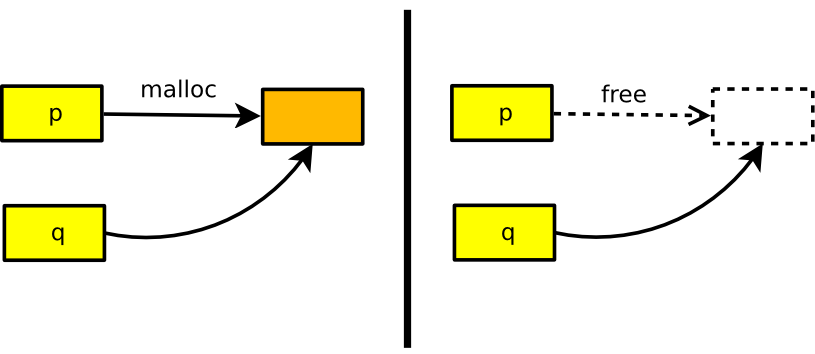
\includegraphics[width=.85\linewidth]{images/dangling}\\
%{\centering \Large Memory Leak}
%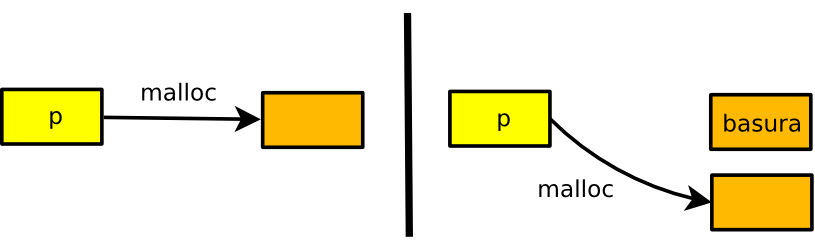
\includegraphics[width=.85\linewidth]{images/lostheap}
%\end{center}
%}
%
%\frame[containsverbatim]
%{
%\frametitle{Ejemplo}
%
%\begin{center}
%{\centering \Large Dangling}
%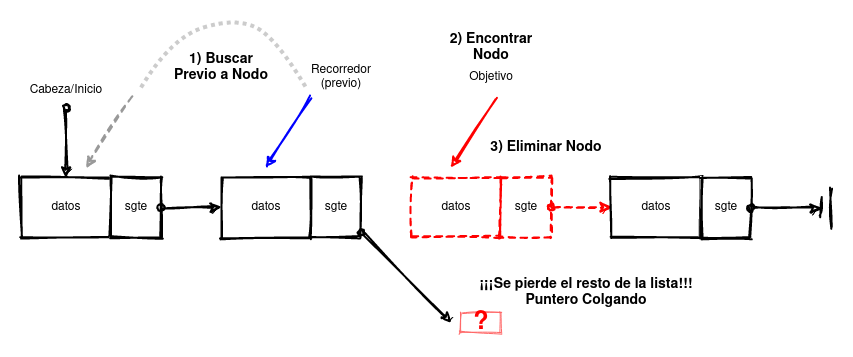
\includegraphics[width=.85\linewidth]{images/listdangling}\\
%{\centering \Large Memory Leak}
%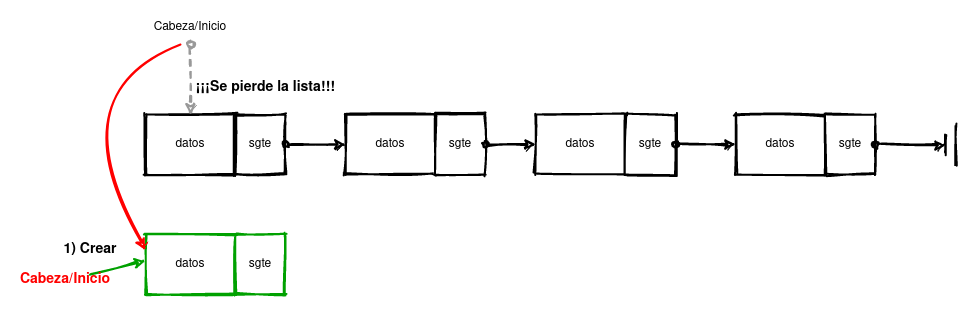
\includegraphics[width=.85\linewidth]{images/listmemoryleak}
%\end{center}
%}
%
%\section{Mejora: Lista enlazada PRO}
%\begin{frame}[fragile]
%\frametitle{Lista Enlazada PRO}
%Existen otras implementaciones de listas enlazadas simples, donde se incluyen más punteros y variables de control.
%
%\begin{exampleblock}{C}
%\begin{lstlisting}[language=C, basicstyle=\tiny, escapeinside={|}{|}]
%#include<stdio.h>
%
%typedef struct nodo{
%	int dato; //dato, puede ser lo que uds. necesiten
%	struct nodo *sgte; // puntero a un nodo enalce.
%} nodo_t;
%
%typedef struct list{
%	nodo_t * inicio;
%	nodo_t * final;
%	int largo;
%} lista;
%
%int main(int argc, char **argv){
%	lista *L = malloc(sizeof(lista));
%	L->inicio = NULL;
%	L->final = NULL;
%	L->largo = 0;
%	// Equivalente a lista vacía []
%	// ¿Para que sirve esta nueva forma?
%	// Implemente las funciones de ésta clase considerando esta forma.
%
%	free(L);
%	return 0;
%}
%\end{lstlisting}
%\end{exampleblock}
%\end{frame}
%
%\begin{frame}[fragile]
%\frametitle{Lista Enlazada PRO}
%\begin{center}
%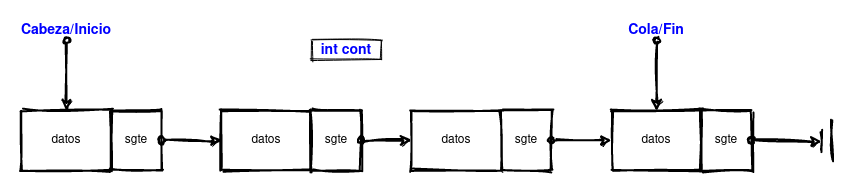
\includegraphics[width=.9\linewidth]{images/linkedlist2}
%\end{center}
%
%
%\begin{center}
%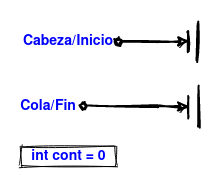
\includegraphics[width=.25\linewidth]{images/init2}
%\end{center}
%
%\end{frame}
%
%
%\section{Ejercicio: Construyendo la lista de Python en C}
%\begin{frame}[fragile]
%\frametitle{Lista de Python en C}
%
%Implemente una lista, para algún tipo de dato a su elección, que incluya las funciones más conocidas de las listas de Python:
%
%\begin{itemize}
%\item \texttt{list()} o \text{[]}.
%\item \texttt{.insert(pos, value)}
%\item \texttt{.append(value)}
%\item \texttt{.clear()}
%\item \texttt{del lista[pos]}
%\item \texttt{.remove(value)}
%\item \texttt{.sort()}
%\item \texttt{.reverse()}
%\item \texttt{.count(value)}
%\item \texttt{.index(value)}
%\end{itemize}
%
%\end{frame}

\end{document}
